\documentclass[10pt,a4paper]{report}
\usepackage[utf8]{inputenc} 
\usepackage[spanish]{babel}
\usepackage{amsmath}
\usepackage{amsfonts}
\usepackage{amssymb}
\usepackage{graphicx}
\usepackage{multirow}
\usepackage{geometry}
\usepackage{fancyhdr}
\usepackage{hyperref}
\usepackage{natbib}

% Márgenes
\geometry{top=2.5cm, bottom=2.5cm, left=3.0cm, right=2.5cm}

%Cabecera y pie de página
\pagestyle{fancy}
\lhead{\rightmark} % texto izquierda de la cabecera
\chead{} % texto centro de la cabecera
\rhead{} % número de página a la derecha
\lfoot{Antonio Molina García-Retamero}
\cfoot{}
\rfoot{\thepage}

% Interlineado
\renewcommand{\baselinestretch}{1.5}


\author{Antonio Molina García-Retamero}
\title{Optimización de redes neuronales mediante métodos bioinspirados}
\makeindex
\begin{document}
\onecolumn
\maketitle
\pagebreak
\tableofcontents
\pagebreak

\chapter{Introducción}
\section{La propuesta de Trabajo de Fin de Grado}
En este documento se recoge la memoria del trabajo de fin de grado que he realizado y que pretende justificar los valores y facultades adquiridas en el estudio y superación de las competencias recogidas en el Grado en Ingeniería Informática. En estas primeras líneas trataré de exponer el trabajo en términos generales y justificar la elección del mismo y las bondades y problemas del mismo.

\subsection{Justificación y objetivos}
En el proceso de elección del proyecto de fin de grado y de los objetivos a plantear para el desarrollo del mismo, he de indicar que primó mi clara vocación investigadora y es por ello que desde el principio le planteé a mi tutor del proyecto mi deseo de realizar algún tipo de investigación básica, con especial interés es el campo de la inteligencia artificial. Es por eso que este proyecto de fin de grado está generalmente enfocado al desarrollo de una investigación que pueda encontrar una aplicación práctica evidente y que cubra en la medida de lo posible todas las competencias adquiridas durante el grado. Por lo tanto, los objetivos generales que cubren este trabajo serían:
\begin{itemize}
	\item Búsqueda de un problema relativo al campo de estudio sobre el que realizar un proceso investigador con tal de dar solución al problema desde un punto científico-técnico.
	\item Estudio del estado del arte del problema en cuestión.
	\item Planteamiento de soluciones.
	\item Experimentación.
\end{itemize}

La redacción de esta memoria está estructurada haciendo una división entre el trabajo puramente teórico e investigador que será la primera parte de la misma y que tratará de clarificar la metodología de investigación, el planteamiento del problema objeto de estudio y el estudio del estado del arte. En la segunda parte se tratará el diseño y la implementación del banco de pruebas sobre el que realizar el proceso experimentador y se justificará la elección de las tecnologías y metodologías utilizadas. En la tercera parte de esta memoria se detallará la experimentación realizada, se recogerán los resultados y se detallarán las conclusiones del trabajo en su conjunto. 

\chapter{Proceso de investigación}
\section{Planteamiento del problema}
Una vez definido el trabajo y planteados los objetivos de este trabajo fin de grado, el siguiente paso ha sido determinar el problema que se va a tratar dentro del proceso investigador y así tratar de proponer una solución al problema siguiendo una metodología de investigación.
Las redes neuronales artificiales han pretendido, desde su concepción, emular, de alguna manera, el proceso cognitivo que se produce en el cerebro de los mamíferos, siempre a una escala reducida, pero sirviéndose de los mismos principios fundamentales. Sin embargo, el problema del aprendizaje es tradicionalmente objeto de la estadísticas y no de la biología. Las redes neuronales artificiales aplicadas al problema de aprendizaje han sido muy estudiadas como un problema estadístico y existe una muy extensa literatura al respecto, sin embargo, no ha sido hasta años recientes que se está abordando el problema del aprendizaje máquina desde un punto de vista biológico. En los últimos años, la neurocomputación ha adquirido una muy notable importancia dentro del campo del aprendizaje máquina y propone sistemas que realmente pretenden emular a los sistemas biológicos y en los que la posibilidad de llegar a entender quizá un poco más los procesos que dotan a los sistemas biológicos de inteligencia y quizá incluso emular algunas de sus funcionalidades es un campo muy prometedor y cargado de retos ilusionantes.

Partiendo del problema de tratar de emular mecanismos biológicos en los modelos de aprendizaje máquina, mi tutor, Daniel Ruiz, me mostró el trabajo de Diego Andina sobre la aplicación de la metaplasticidad neuronal al perceptrón multicapa (MLP) y me propuso aplicarlo a otro tipo de redes como las RBFN.

\section{El estado del arte}
Dado que partimos de un trabajo en curso, que es la implementación de la metaplasticidad artificial en redes neuronales artificiales, el estudio del estado del arte ha sido un trabajo aurduo que ha requerido de un estudio bastante en profundidad de las diferentes disciplinas bajo las que se contempla el problema que hemos definido y que cubren desde la neurobiología a la estadística y el aprendizaje máquina. Es por esto que me serviré de esta sección primero para demostrar de alguna forma el trabajo realizado en la documentación y adquisición de conocimientos necesarios para comprender el problema y plantear una solución así como para tratar de introducir al lector, de la forma más amena posible, en los conceptos y terminología en que se definen la problemática y la solución propuesta al problema.

El trabajo se inicia con el estudio de lo relativo a la metaplasticidad en las redes neuronales biológicas. Además, he dedicado tiempo a estudiar y entender los modelos estadísticos bajo los que se estudian las redes neuronales artificiales para buscar la forma de aplicar este principio, que es la metaplasticidad artificial, a otros tipos de redes neuronales artificiales más allá, y partiendo, del trabajo que ha desarrollado Diego Andina en las MLP.

Una vez adquiridos los conocimientos necesarios para comprender el problema, se realizará un estudio del estado del arte de las diferentes técnicas de las RBFN con tal de encontrar la forma de aplicar el concepto de metaplasticidad que se da de forma natural en las redes neuronales biológicas.

En las siguientes subsecciones se definirán primero la metaplasticidad en términos biológicos y se expondrá la propuesta de Diego Andina para poder especificar el problema y, partiendo de ahí, plantear la solución propuesta. 

En este punto de la investigación se ha recurrido de nuevo a la bioinspiración tratando de encontrar una perspectiva bajo la que contemplar las RBFN y sobre la que plantear una solución al problema. 

\section{La metaplasticidad en redes biológicas}
Con el término metaplasticidad nos referimos al cambio dependiente de la actividad que modula la plasticidad sináptica en los sistemas neuronales. Estos cambios en la plasticidad pueden ser del tipo LTP\footnote{\textbf{Long-Term Potentiation} es la potenciación de la eficiencia provocada por los eventos más reciente en la señal transmitida entre dos neuronas que se estimulan síncronamente} y LTD\footnote{\textbf{Long-Term Depression} es la reducción de la eficiencia provocada por los evento menos reciente en la señal transmitida entre dos neuronas que se estimulan síncronamente}. Abraham and Bear lo definió de forma sencilla como: \textit{plasticity of synaptic plasticity}, es decir, la plasticidad de la plasticidad sináptica. A diferencia de los mecanismos convencionales de neuromudalación de la plasticidad sináptica en los que son neurotransmisores y hormonas los que inducen cierto grado de LTP y LTD, la metaplasticidad se refiere al cambio que es provocado en un momento dado por lo que comunmente denominamos \textit{primar} la actividad. Es decir, la metaplasticidad se refiere a la inducción en los cambios de los LTP y LTD derivados de la actividad. Reforzando aquellas conexiones sinápticas relativas a las \textit{experiencias} más comunes y deprimiendo aquellas relativas a \textit{experiencias} menos comunes.

Funcionalmente, la metaplasticidad dota a las conexiones sinápticas de la capacidad de integrar señales relativas a la plasticidad a través del tiempo. Además, la metaplasticidad tiene un importante papel como regulador de los umbrales de los LTP y LTD para mantener las conexiones sinápticas en un rango funcional dinámico que evite que estas conexiones se vuelvan demasiado fuertes o demasiado débiles como consecuencia de los mecanismos de plasticidad sináptica convencionales basados en neurotransmisores y hormonas.

\section{Metaplasticidad en redes neuronales artificiales}
El doctor Diego Andina realizó una aproximación a la integración de los mecanismos de metaplasticidad en ..., donde se propone un mecanismo de metaplasticidad artificial (AMP\footnote{Artificial Metaplasticity}) aplicado a las MLP\footnote{Multilayer Perceptron}. En las siguientes líneas trataré de explicar la interpretación que Diego Andina propone sobre la metaplasticidad en el cálculo del error y de la modificación del algorítmo de \textit{backpropagation} propone para la implementación de la AMP en los MLP.

El problema del entrenamiento en cualquier problema de aprendizaje es el de minimizar una función de error ajustando los parámetros del modelo en base a un conjunto de vectores de entrada $x=(x_1,x_2,...,x_n),(x\in\Re^n)$ que conforman el \textit{training set}. En base al criterio de error $E(x)$ que elijamos, el error esperado del sistema será por tanto:
\begin{equation}
	E_M = \int_{\Re^n}E(x)f(x)dx = \int_{\Re^n}e(x)dx
\end{equation} 
Sobre lo que podemos hacer la siguiente transformación:
\begin{equation}
	\label{metaSub1}
	E_M = \int_{\Re^n}\dfrac{e(x)}{f^*_X(x)}f^*_X(x)dx = \varepsilon^*\lbrace\dfrac{e(x)}{f^*_X(x)}\rbrace
\end{equation}
y calcular el error del modelo añadiendo el siguiente estimador:
\begin{equation}
	\label{metaSub2}
	\widehat{E}_M=\dfrac{1}{M}\sum^M_{k=1}\dfrac{e(x^*_k)}{f^*_X(x^*_k)}
\end{equation}
donde $x^*_k,k=1,2,...,M$ son muestras independientes cuya $pdf$ es $f^*_X(x)$. Como se observa, $f^*_X(x)$ es la distribución de probabilidad de la función que tratamos de generalizar con nuestro modelo a través de nuestras muestras de entrenamiento. Por lo tanto, idealmente, 
\begin{equation}
	\label{metaSub3}
	(f^*_X(x))_{opt}=\dfrac{1}{E_M}e(x)
\end{equation}

Lo que se pretende conseguir a través de la introducción de la función subóptima de las ecuaciones \ref{metaSub1} y \ref{metaSub2} es incluir el factor de probabilidad a posteriori de la muestra con tal de provocar un efecto de LTP o LTD en los pesos sinápticos consiguiendo así introducir un mecanismo de metaplasticidad en la red neuronal artificial.
Como se expresa en la ecuación \ref{metaSub3}, la función $f^*_X(x)$ óptima sería la $pdf$ de la señal de entrada de nuestro modelo ($f_X(x)$), lo que es desconocido por nosotros, con lo que, en la práctica, se elige una $f^*_X(x)$ arbitraria tal que $f^*_X(x) \simeq f_X(x)$.

La figura \ref{fig:WeightedTrainEpoch} ilustra como se incorpora el mecanismo de metaplasticidad como un factor de corrección sobre los pesos. Como se observa, esta corrección del error se hace en base a la salida esperada siendo esta, como ya hemos dicho, $f^*_X(x)$.

\begin{figure}[h!]{}
    \centering
    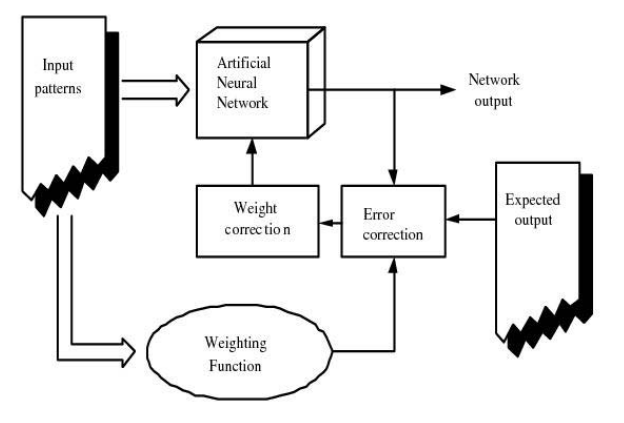
\includegraphics[width=0.6\textwidth]{img/weightingOperation.png}
    \label{fig:WeightedTrainEpoch}
    \caption{Iteración en el entrenamiento de una red neuronal aplicando el mecanismo de metaplasticidad}
\end{figure}


\subsection{Propuesta de implementación de la AMP en las MLP}
En base a esta interpretación que Diego Andina hace de la metaplasticidad en el mismo artículo \citep{Andina2009} se propone la siguiente modificación sobre el algoritmo de \textit{backpropagation} para incluir la función subóptima $f_X(x)$ a los MLP. 
\begin{equation}
	\dfrac{\partial\varepsilon(W)}{\partial w^{(S)}_i} = \dfrac{\partial}{\partial w^{(S)}_i}\left(\dfrac{1}{2}\dfrac{(y-\widehat{y}^{(S)})^2}{f^*_X(x)}\right) = \dfrac{1}{f^*_X(x)}\dfrac{\partial\varepsilon(W)}{\partial w^{(S)}_i}
\end{equation} 
\begin{equation}
	\label{eqErrorLastLayer}
	\delta_j^{(S)} = (y_j - \widehat{y}^{(S)}_j) \cdot \dfrac{f^{'(S)}}{f^*_X(x)}
\end{equation}
siendo s el contador de capas, $s=1,2,...,S$, $j$ e $i$ son el contador de nodos y entradas y $\delta_j^{(S)}$ el error de un nodo $j$ para la capa $s$. Por tanto, la ecuación \ref{eqErrorLastLayer} define el cálculo del error para los nodos de la última capa. Para el resto de capas, el error se propaga siguiendo la forma convencional del \textit{backpropagation}.
En definitiva, lo que se propone es incluir para, cada iteración en el entrenamiento, es ponderar ese peso en un factor que es el siguiente:
\begin{equation}
	w^*(x) = \dfrac{1}{f^*(x)}
\end{equation}
con lo que se consigue acelerar el entrenamiento dando más importancia a los casos menos frecuentes. Esto además es acorde con la teoría de la información en tanto que \textit{los sucesos menos frecuentes contienen más información}.

De todo lo comentado anteriormente, queda patente que una de las claves en la implementación de la metaplasticidad a las redes neuronales es la elección acertada de la función subóptima $f_X(x)$. En el caso concreto de las MLP, para clasificar $L$ clases $H_l$ para $l=0,1,...,L-1$, y basándonos en el teorema de Bayes, obtenemos
\begin{equation}
	\widehat{y}_l \simeq P(H_l/x)=\dfrac{f_X(x/H_l) \cdot P(H_l)}{f_X(x)}
\end{equation}
si asumimos la salida de nuestra red $\widehat{y}_l$ como $P(H_l/x)$, la propia salida de la red neuronal generaliza $f_X(x)$ con lo que esta puede ser utilizada como función subóptima.

De esta forma, Diego Andina obtiene los resultados de la figura \ref{fig:andinaResults} y que representa la media del error para redes con la modificación propuesta (BPW) para un número creciente de operaciones en contraposición con la media del error en redes entrenando con un algorítmo de \textit{backpropagation} tradicional(BP). En este caso, la función de distribución de probabilidad, se ha asumido la siguiente gaussiana
\begin{equation}
	f^*_X(x) = \dfrac{A}{\sqrt{(2\pi)^n} \cdot e^{\dfrac{B}{8} \sum_{i=1}^n{x_i^2}}}
\end{equation}
donde $A$ y $B$ son los parámetros de la gaussiana que en este caso representan los parámetros de la metaplasticidad. En el artículo\citep{Andina2009} se muestra el siguiente ejemplo de como puede mejorar esta propuesta para una entrada concreta en un escenario, se supone, ideal:

\begin{figure}[h!]{}
    \centering
    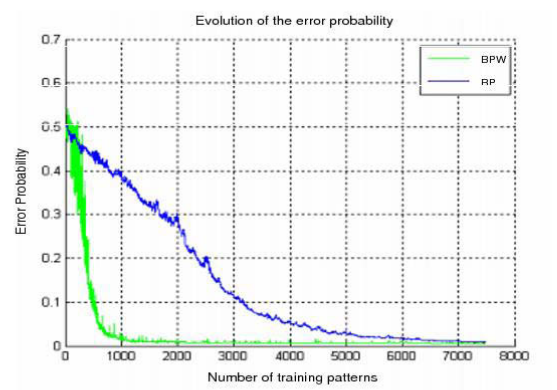
\includegraphics[width=0.6\textwidth]{img/ArticleResults.png}
    \label{fig:andinaResults}
    \caption{Comparación de la evolución del aprendizaje del algorítmo ponderado (BPW) frente al tradicional (BP)}
\end{figure}

\subsubsection{Implementación propia}
Sobre esta propuesta de modificación del algorítmo de \textit{backpropagation} realicé mi propia implementación con tal de poder hacer mi propia experimentación. Esta implementación la basé en el desarrollo de una MLP que realicé para la asignatura de \textit{Razonamiento Automático} en C++. El objetivo de esta implementación era tan solo el de poder experimentar de primera mano, utilizar diferentes funciones subóptimas y diferentes datos de entrenamiento. 
Así, en la siguiente subsección expondré las conclusiones derivadas del estudio y la experimentación de la técnica propuesta por Diego Andina.
 Esta implementación está publicada en el siguiente repositorio de \href{https://github.com/aydevosotros/AMMLP}{GitHub}\footnote{https://github.com/aydevosotros/AMMLP}.

\fbox{Esto creo que se me queda corto, pero tampoco se muy bien que más decir}

\subsubsection{Conclusiones del estudio}
Una vez asimilados los conceptos y habiendo realizado una implementación y haber experimentado primero sobre el conjunto de datos sobre los que se publica el artículo y después con otros conjuntos de datos públicos y típicos en los problemas de aprendizaje máquina y habiendo experimentado con diferentes funciones subótimas, he alcanzado las siguientes conclusiones
\begin{itemize}
	\item Encontrando una función subóptima que se aproxime a la función de distribución de probabilidad de los datos que componen la señal de entrada podemos obtener una gran mejora emulando los procesos LTP y LTD de los sistemas biológicos.
	\item A priori, $f_X(x)$ es desconocida en los problemas de aprendizaje máquina, con lo que escoger una $f^*_X(x)$ subótima apropiada es un problema muy considerable.
	\item La posibilidad de aproximar $f_X(x)$ por la salida de la red neuronal $\widehat{y}_l$ cuando esta está lo suficientemente entrenada como para proveer una aproximación lo suficientemente buena puede ser muy interesante.
\end{itemize}

\section{Metaplasticidad Artificial en RBFN}
En esta sección trataré de expresar la problemática observada en el proceso de encontrar y aplicar algún mecanismo de metaplasticidad artificial aplicado a las redes neuronales con función de activación de base radial (RBFN). Para ello, haré en primer lugar una breve introducción a las RBFN tratando de introducir al lector en las principales características de este tipo de redes para después exponer una primera solución y la problemática encontrada.
\subsection{Definición y características de las RBFN}
Para el estudio de las RBFN, fundamentalmente he estudiado el libro de \textit{Simon Haykin}\cite{haykin99a}. 

\begin{figure}[h!]{}
    \centering
    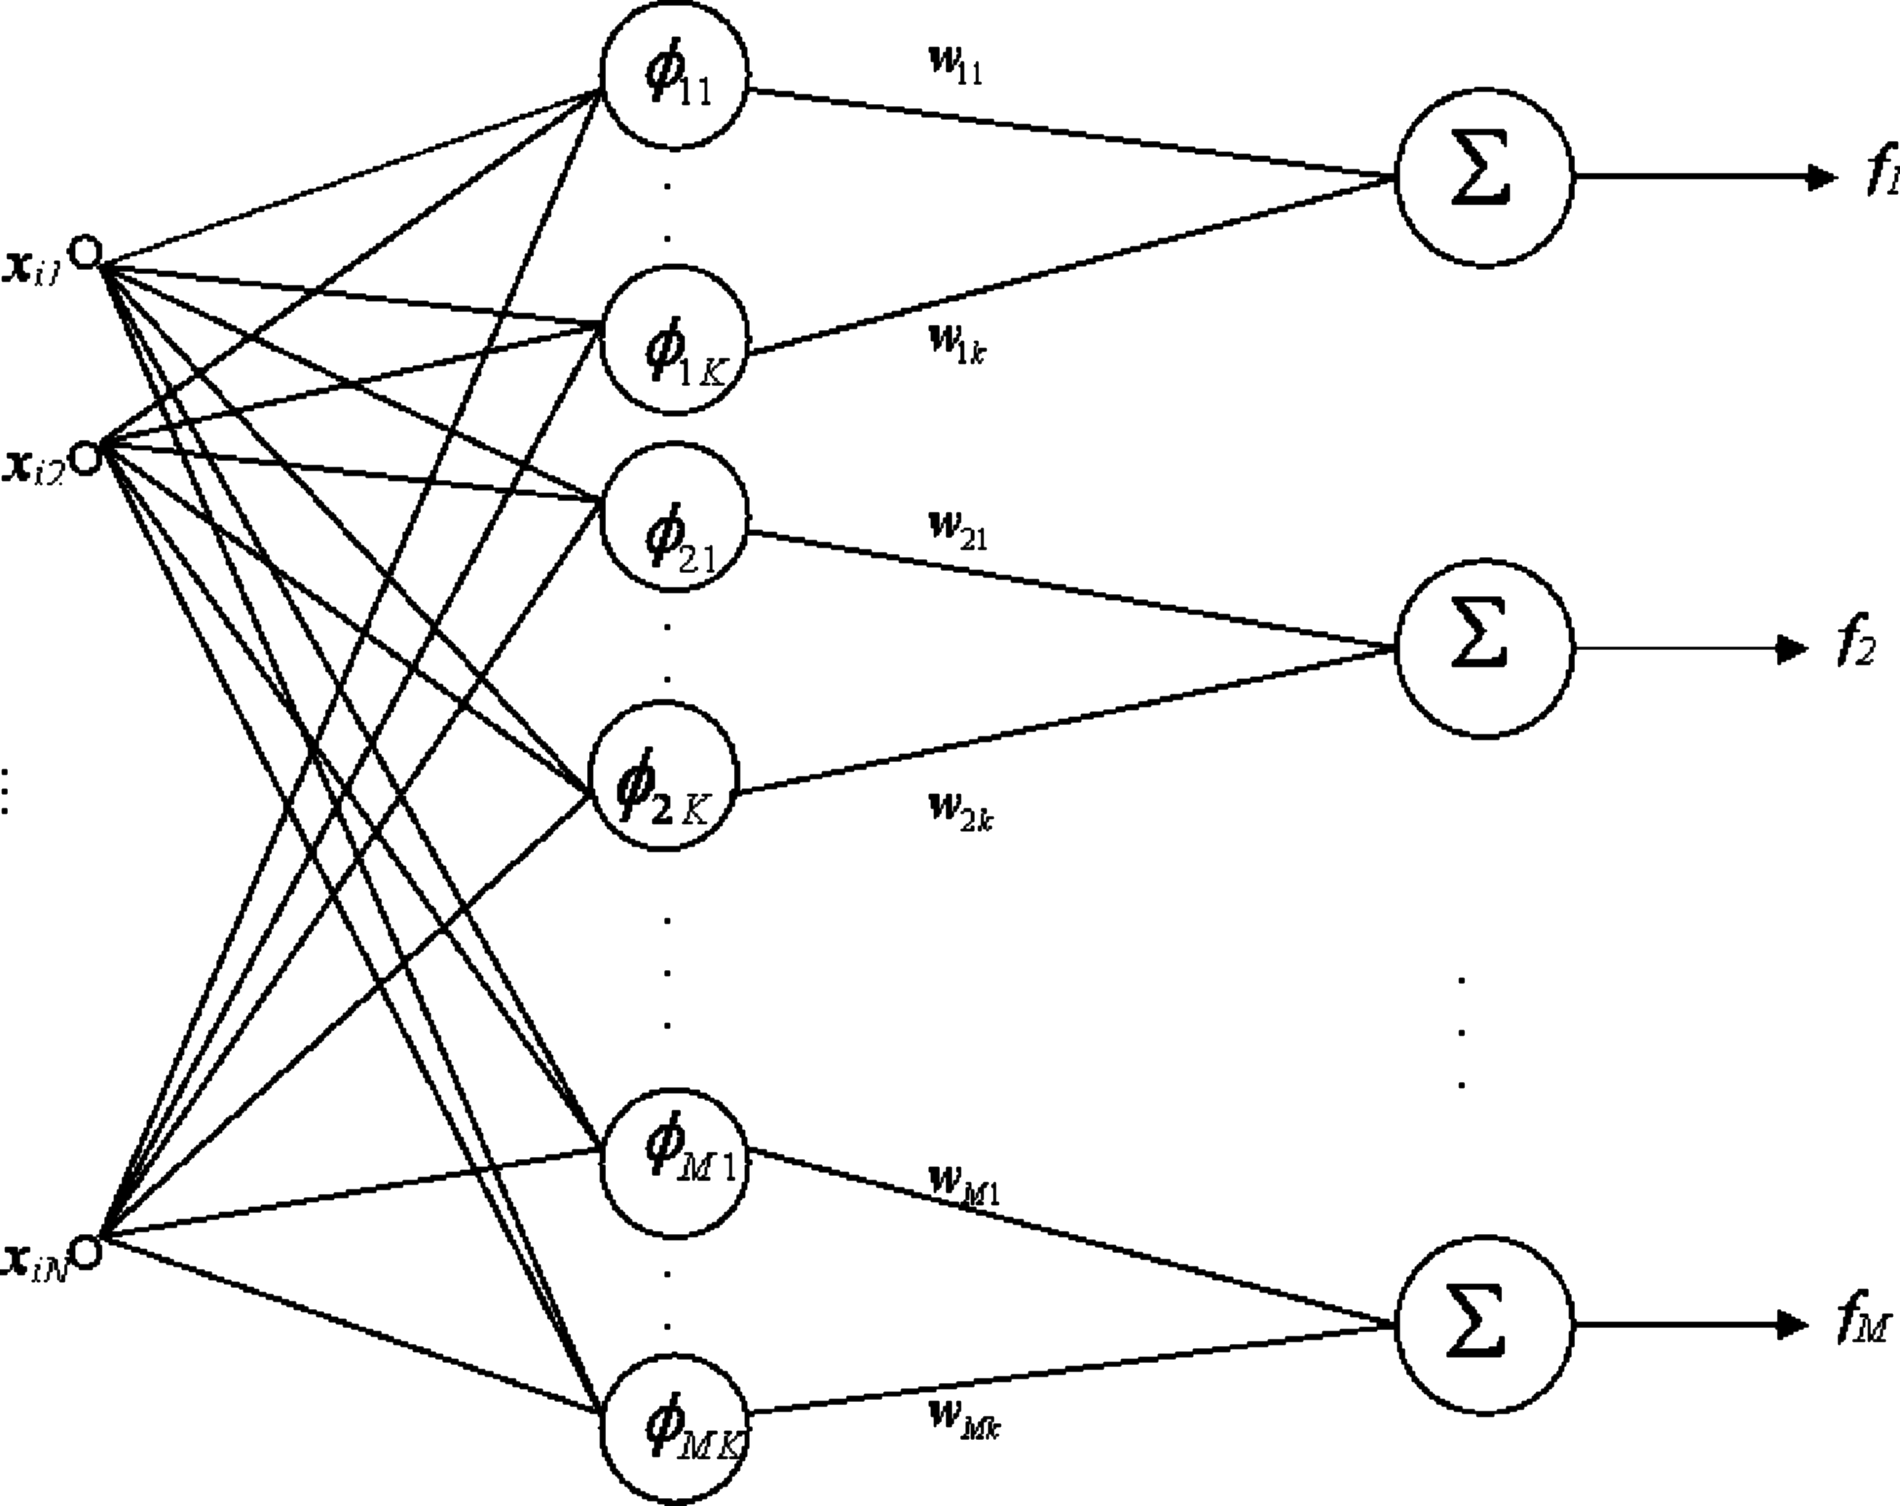
\includegraphics[width=0.6\textwidth]{img/RBFN1.png}
    \label{fig:RBFN1}
    \caption{Arquitectura de las RBFN}
\end{figure}

\subsubsection{Metodologías de entrenamiento}
\subsection{Aplicación directa del estimador de probabilidad}
Una primera implementación de la metaplasticidad en las RBFN podría ser la de incluir la estimación de probabilidad subóptima en la fase de entrenamiento de pesos con tal de ponderarlos de forma similar a, como explicado, Diego Andina propuso para las AMMLP\citep{Andina2009}.

De la misma forma que explicamos anteriormente, 
\begin{equation}
	E_M = \int_{\Re^n}{e(x)dx}
\end{equation}
hacemos igualmente la transformación con tal de incluir el estimador $f^*_X(x)$
\begin{equation}
	\label{metaRBFN1}
	E_M = \int_{\Re^n}\dfrac{e(x)}{f^*_X(x)}f^*_X(x)dx = \varepsilon^*\lbrace\dfrac{e(x)}{f^*_X(x)}\rbrace
\end{equation}
para obtener de nuevo el error del sistema en función del criterio de error que elijamos $e(x^*_k)$ y la función de distribución de probabilidad $f^*_X(x)$
\begin{equation}
	\label{metaRBFN2}
	\widehat{E}_M=\dfrac{1}{M}\sum^M_{k=1}\dfrac{e(x^*_k)}{f^*_X(x^*_k)}
\end{equation}

\subsubsection{Propuesta de implementación}
Para aplicar este nuevo cálculo del error a una RBFN, tan solo hemos de aplicar el criterio de error a la propia red. Si consideramos el criterio de error más típico que es el del cuadrado de la diferencia e incluyéndolo en \ref{metaRBFN2} obtenemos:
\begin{equation}
	\label{metaRBFN3}
	\widehat{E}_M=\dfrac{1}{M}\sum^M_{k=1}\dfrac{(y_k - \overbrace{\left(\sum^M_{j=1}{w_j G(\Vert x^*_k - t_j \Vert_{C_j})}\right)}^{Salida\ de\ la\ RBFN})^2}{f^*_X(x^*_k)}
\end{equation}
que sustituiremos la derivada parcial respecto $w_i$
\begin{equation}
	\dfrac{\partial\varepsilon(n)}{\partial w_i(n)} = \sum^N_{j=1}{\widehat{E}_M(n) G(\Vert x_j - t_i \Vert_{C_i})}
\end{equation}
Por tanto, y en términos del algorítmo general, el entrenamiento de nuestra RBFN solo cambia con respecto a las técnicas de entrenamientos típicas con la única variación de que la función de coste será la definida en \ref{metaRBFN3}
\begin{equation}
	w_i(n+1)=w_i(n) - \eta \dfrac{\partial\varepsilon(n)}{\partial w_i(n)}
\end{equation}

\subsection{Problemática}
Una vez asumido el concepto de metaplasticidad en las redes neuronales biológicas y partiendo de la propuesta de metaplasticidad artificial en las MLP de Diego Andina, estamos en disposición de abordar el problema. 
Como ya se ha expuesto anteriormente y en esencia, la propuesta de Diego Andina se basa en la emulación de los procesos LTP y LTD añadiendo un factor que pondera la derivada parcial en el descenso por gradiente de la muestra con respecto al peso de la conexión sináptica que representa cuan \textit{raro}, en términos de probabilidad, es la muestra respecto a la clase en que se clasifica a posteriori. Esta probabilidad a posteriori se estima por la propia salida de la red neuronal en ese estado del entrenamiento. 

En este punto, queda patente que existe numerosos problemas a la hora de aplicar esta técnica a otro tipo de redes neuronales, en particular en las RBFN. En la figura \ref{fig:RBFN1}, se representa la arquitectura típica de una RBFN.

Un problema fundamental se debe a la salida de la última capa de sendas redes neuronales. Para implementar un mecanismo de metaplasticidad similar al descrito en las AMMLP, se requiere de una estimación de la probabilidad de pertenencia a la clase (cuan \textit{rara} es la muestra) y en las AMMLP la estimamos como la salida de la propia red neuronal. Ya que la neurona de la última capa es una función logística \footnote{Una función logística es una función continua cuya salida $\in [0 1]$. Un ejemplo de función logística típia es \\ $f_{log}(z)=\frac{1}{1+e^{-z}}$}, asumimos ésta como la probabilidad a posteriori de pertenencia a la clase. Por su parte, la salida de una RBFN para el problema de clasificación se calcula como $sign(f(x)=\sum w \phi(x))$. Queda patente que la salida de la RBFN no nos sirve para estimar una probabilidad a posteriori de la muestra.

Sin embargo, la propia naturaleza de las RBFN parece resultar idónea a su vez para experimentar con técnicas. Este \textit{parecer} es una percepción completamente intuitiva, pero existen ciertas características que trataré de explicar a continuación que pueden hacer de estas redes idóneas para representar las redes neuronales biológicas y a la forma en que estas representan la información y que me inspiraron a plantearme el problema en multitud de formas tratando de encontrar la forma de encajar estas características con la naturaleza del aprendizaje y de la metaplasticidad. Estas características son, en líneas generales:

\begin{itemize}
	\item La capa oculta característica de las RBFN está compuesta por \textit{neuronas} cuya función de activación es típicamente una gaussiana en la forma . Estas gaussianas tienen dos parámetros básicos y que son fundamentalmente dependientes de la naturaleza de la señal de entrada y que son un centroide y la varianza.
	\item La capa oculta, a su vez, realiza una transformación no lineal en un espacio basado en la distancia. Esta característica sirve de nexo para el estudio de las RBFN dentro del conjunto de los \textit{Kernel Methods}.
	\item La matriz de covarianza determina el campo receptivo de las funciones de activación de base radial gaussianas.
\end{itemize}

Expuestos los problemas y las caracterísitcas más relevantes en este estudio, continué la investigación buscando técnicas a través de las cuales poder extraer información que pudiera estimar la función de distribución de probabilidad de la señal de entrada. Tal y como hemos visto anteriormente, existen típicamente dos fases de entrenamiento y en la primera de estas se trata de encontrar la posición de los centroides en el espacio de características para las gaussianas de la capa oculta y, en ocasiones, estimar una covarianza para estas gaussianas. Esta primera fase es, por tanto y básicamente, una búsqueda de información sobre la señal de entrada donde tratar de estimar de alguna forma $f_X(x)$ y utilizarlo en la segunda fase de entrenamiento para ponderar los pesos con la función $w^*$ en un descenso por gradiente en busca de minimizar la función de coste de nuestra red.

\section{Ampliación del estado del arte}

\subsection{Tonotopía y Retinotopía}
\subsection{Kernel Methods}
\section{Propuesta de solución}
En base a los trabajos previos, la idea de servirnos de la naturaleza de los datos de nuestro entrenamiento para hacernos una idea a priori de cuan significativa es una muestra y actuar ponderando esa "conexión sináptica" concreta parece encajar de forma especial en el concepto de RBFN debido a la naturaleza de las Funciones de Base Radial. Quiero decir, las Funciones de Base Radial nos proporcionan una transformación no lineal que nos permite encontrar un hiper-plano que en algún espacio multidimensional nuestros datos serán separables. El modelo de las RBFN, como ya hemos comentado, se sirven de un modelo con la forma $f(x)=\sum w \phi(x)$ donde $\phi(x)$ es un función de base radial. Este tipo de funciones pueden ser muy variadas y se ha experimentado con multitud de ideas alrededor de esto sin embargo en los casos más habituales se utiliza una función gaussiana en donde tenemos que inferir tanto la media como los centroides para cada una de las funciones en nuestro conjunto de datos. De esto se deriva un entrenamiento de dos fases en el que en la primera fase inferimos los datos necesarios para calcular la activación de la capa oculta para hacer luego encontrar los parámetros para la transformación lineal sobre la salida de esta capa en una segunda fase de entrenamiento.

Aquí es donde pretendo encontrar y probar diferentes formas de optimizar la segunda fase de entrenamiento sirviéndonos del estudio estadístico que implica la primera fase. Esto es, Cuando en la primera fase de entrenamiento buscamos los centros para nuestras funciones de activación obtenemos información relevante que podemos utilizar para estimar, como hablábamos antes, como considerar una probabilidad de pertenencia a una clase si consideramos el centroide como una clase, etc... Multitud de ideas se pueden considerar y en última instancia lo que se estaría haciendo sería entremezclar de diferentes formas el proceso de aprendizaje no supervisado a priori para influir en el proceso de aprendizaje supervisado de la segunda fase.


\chapter{Implementación}
Con tal de dar soporte al planteamiento teórico que ha sido expuesto en la sección anterior, he desarrollado un \textit{benchmarks} sobre el que realizar la experimentación que sustente la validez (o pruebe la falta de esta) de los algoritmos propuestos. Pese a tener un objeto muy concreto, he tratado de realizar un diseño tan generalista como me fuera posible, tratando de definir y delegar las responsabilidades entre clases y persiguiendo siempre un bajo acoplamiento y una alta cohesión entre estas.
En líneas generales, el software desarrollado ha de cubrir los siguientes objetivos:
\begin{itemize}
	\item Implementar una \textbf{RBFN} configurable tanto en los parámetros propios de la RBFNN (dimensionalidad, parámetros de las gaussianas, etc...) como en los algorítmos de entrenamiento.
	\item Implementar un mecanismo de \textbf{generación/obtención} de los conjuntos de datos:
	\begin{itemize}
		\item Ha de ofrecer la posibilidad de generar datos aleatorios en base a una \textit{fdp} ($f_X(x)$) conocida con tal de facilitarnos la experimentación en nuestro problema en concreto en el que, como se ha discutido ampliamente en secciones anteriores, esta función tiene un papel fundamental.
		\item Además, ha de ofrecer diferentes conjuntos de datos reales con tal de posibilitar la experimentación y comparación de estos algoritmos con el estado del arte del problema.
	\end{itemize}
	\item Implementar un mecanismo que recopile los resultados obtenidos y \textbf{genere un informe} con toda la información necesaria para evaluar estos resultados
\end{itemize}

Una vez especificados los objetivos, en las siguientes subsecciones describiré y justificaré las metodologías escogidas para el desarrollo del software. Además, describiré y justificaré la elección del lenguaje de programación escogido y de las herramientas en las que me he apoyado para el desarrollo. Por último, trataré de ir describiendo los diferentes paquetes que he desarrollado para cubrir cada uno de los requerimientos que se han planteado en forma de objetivos \textit{(RBFN, Generador de datos, Generador de informes)}

El objetivo final del software a desarrollar es el de proveer de un \textit{framework} de desarrollo rápido que fuera lo más general y flexible posible para poder realizar una experimentación lo más rápida y cómoda posible. Es decir, el objetivo último era conseguir un entorno con las siguientes características:
\begin{itemize}
	\item \textbf{Flexible:} 
	\item \textbf{Extensible:}
	\item \textbf{Desarrollo rápido:}
\end{itemize}


\section{Metodología de desarrollo}
En cuanto a las metodologías de desarrollo, en fase de diseño, determiné usar diferentes metodologías para afrontar los diferentes problemas y con tal de aprovechar las ventajas que, sobre cada uno de los problemas, estas ofrecen.

Así pues, para implementar la RBFN me serví de un desarrollo basado en Test Driven Development (TDD). Debido a la complejidad de implementación a la susceptibilidad de errores de implementación en los algorítmos, me aproximé al desarrollo de la red neuronal basándome en diferentes pruebas lo suficientemente sencillas para poder precalcular cada uno de los resultados de los algoritmos y garantizar así la correcta implementación. Así mismo, el diseño de la clase vino determinado por las necesidades que surgían al diseñar las pruebas y que, por lo tanto, siguiendo un desarrollo \textit{up-to-bottom}.

Para el desarrollo del generador de datos realicé un Diseño Orientado a Objetos con un enfoque cercano a la Programación Extrema. Esto es, dado que los requisitos para el generador de datos, descritos anteriormente, me permitían hacer un diseño de clases bastante claro ya que los propios requisitos definen la interfaz pública de la clase generadora de datos (\textit{generarDataSet, obtenerX, obtenerY, etc...}).

Por último, para el generador de informes me serví de una combinación de estas. Es decir, partía de un resultado esperado que era el informe y una interfaz pública más o menos clara (\textit{addGrafico, addSection, etc}). Sin embargo en tiempo de desarrollo, las pruebas fueron redefiniendo esta interfaz en base a los requisitos que iban imponiendo las pruebas rediseñando así el modelo en cada \textit{iteración} del desarrollo.

\section{Lenguaje y herramientas}
\section{Esquema general del diseño}
\section{Implementación de la RBFN}
\section{Implementación del generador de datos}
\section{Implementación del generador de informes}

Dado que por medio de este trabajo se pretende la demostración de la mejora propuesta sobre las RBFN, estableceré una serie de pruebas que pretenderán poner a prueba las diferentes implementaciones de las redes para resolver problemas típicos de aprendizaje máquina.
En secciones anteriores hemos comentado la problemática y las diferentes alternativas propuestas para entrenar las RBFN. La batería de pruebas es la parte probablemente más crítica del proyecto y con especial esmero he diseñado un conjunto de pruebas que pretende ser exhaustivo y con el que pretendo primero valorar el comportamiento de las soluciones típicas existentes y las mejoras propuestas en esta investigación.

De entre los escenarios típicos del aprendizaje máquina podemos hacer dos grandes grupos: tal y clasificación. Para este proyecto he seguido la estrategia de construir, para sendos tipos de problemas, sets de datos aleatorios cuyos parámetros intrínsecos puedan ser manipulados fácilmente permitiendo generar de forma sencilla tantos escenarios como se crean apropiados para los diferentes test. En busca de evitar el "data snooping" y una vez determinadas las configuraciones para los que los diferentes tipos de redes tienen comportamientos interesantes, las redes serán testeados sobre sets de datos estándares en la investigación sobre aprendizaje máquina.

\begin{itemize}
	\item Reconocimiento de patrones
	\begin{itemize}
		\item Onda compuesta aleatoria
		\item Otra idea que se me ocurra
	\end{itemize}
	\item Clasificación
	\begin{itemize}
		\item Clasificación sobre datos aleatorios artificiales
		\item Clasificación sobre datos reales
	\end{itemize}
\end{itemize} 
En las siguientes secciones trataré de clarificar todo esto para cada tipo de pruebas. Explicaré las cosas fundamentales de la implementación tratando de no perder al lector en el código pero dándo una visión clara y precisa de lo que se desea poner a prueba con cada test. Sin embargo, antes de entrar en detalle sobre la construcción de los conjuntos de datos me gustaría dejar patente el guión básico que sigo a la hora de diseñar las prubas.

Anteriormente hemos discutido las fases del entrenamiento de redes RBFN y de las soluciones típicas. Además discutimos acerca de como podemos implementar la intuición de la metaplasticidad en la fase supervisada a partir de la información estadística que supone el aprendizaje no supervisado de la primera parte del entrenamiento en busca de los parámetros de las funciones de base radial. 

Con todo esto, una primera batería de test tratará de determinar en qué condiciones, el cálculo de la pseudoinversa deja de resultar rentable en términos de coste computacional con respecto a al descenso por gradiente. Este coste computacional es directamente proporcional al tamaño del set de datos, con lo que esta prueba nos dará una estimación de cuan grande ha de ser al menos nuestro conjunto de datos para que resulte rentable la aproximación del descenso por gradiente que es necesario para la implementación de la intuición de metaplasticidad aquí propuesta.

A continuación, someteremos a una batería exahustiva de test generados artificialmente y sobre los que variaré los parámetros de los diferentes tipos de redes y de los propios conjuntos de datos en busca de las condiciones en que cada tipo de RBFNs de los propuestos ofrece un comportamiento mejor que el resto. Con esto podremos determinar si existen condiciones en las que, en efecto, la propuesta de metaplasticidad supone una mejora sobre las aproximaciones existentes.

Por último, se realizarán pruebas sobre sets de datos conocidos y ampliamente utilizados en el campo del aprendizaje máquina. Con esto se pretende evitar la aparición de resultados inválidos por la propia intervención y manipulación de los parámetros y datos en busca de las condiciones en las que la esta implementación resulte mejor además de poder ofrecer comparativas que puedan ser reconocidas por quienes trabajan en otras propuestas sobre los mismos conjuntos de datos.

\subsection{Pruebas de clasificación}
Uno de los usos más habituales de las RBFN es cuando tenemos que clasificar sobre un conjunto de datos cuyas clases no son linealmente separables. Anteriormente hablamos de
\begin{figure}[!h]{}
    \centering
    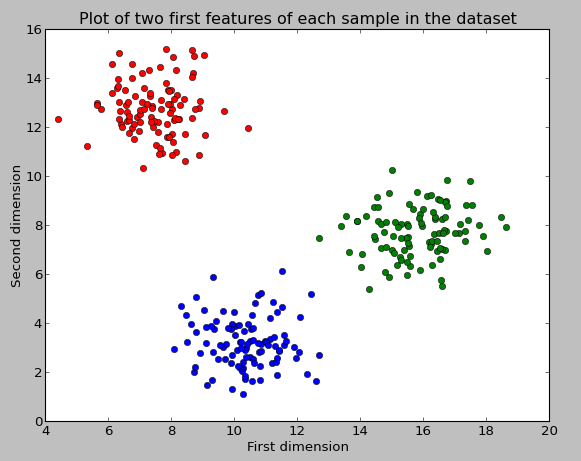
\includegraphics[width=0.4\textwidth]{img/clusteredData1.png}
    \label{fig:clusteredData1}
    \caption{Conjunto de datos con distribución normal}
\end{figure}
Ya que, a través de las RBFN, obtenemos un modelo con la forma $f(x)=\sum w_{i}\phi(r)$ (que es caracterizado con funciones de base radial) podemos aproximar funciones complejas cuya salida sigue una distribución gaussiana (la más frecuente con mucha diferencia de entre las variables aleatorias que se dan en la naturaleza) con notable precisión. 
La figura \ref{fig:clusteredData1} es un ejemplo de datos generados con el generador de datos clusterizados que he implementado. Este recibe como parámetros básicos el número de centroides y el número de muestras y genera estos datos de forma aleatoria tomando como centro los k-centroides también tomados aleatoriamente. En las siguientes líneas introduciré esta clase sin entrar en excesivo detalle de la implementación pero sí tratando de aclarar las cuestiones que considero claves.

\subsubsection{Generación de datos aleatorios}
Para este tipo de test necesitamos generar datos que se distribuyan de forma normal alrededor de un centroide. Una distribución normal es aquella que cuya función de densidad de probabilidad queda definida por la media ($\mu$) y la desviación estándar ($\sigma$) del conjunto de datos ($x$) de la siguiente forma:
\begin{center}
$pdf(x,\mu,\sigma) = \frac{1}{ \sigma \sqrt{2 \pi}} e^{\left(-\frac{{\left(\mu - x\right)}^{2}}{2 \, \sigma^{2}}\right)}$
\end{center} 
Existen multitud de generadores aleatorios de este tipo de datos. En este caso utilizaré el propio de NumPy como muestro a continuación para generar las $n$ muestras por cada centroide ya que este definirá la media. La desviación estándard será proporcionada como parámetro en el constructor de la clase y nos permitirá jugar con la forma que adoptarán los datos generados.

\begin{figure}[!h]{}
    \centering
    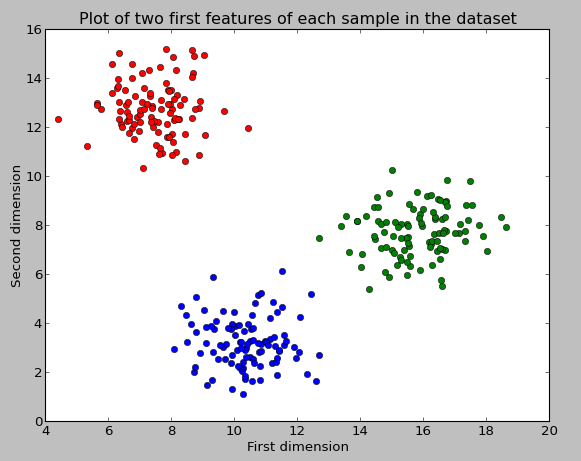
\includegraphics[width=0.4\textwidth]{img/clusteredData1.png}
    \label{fig:clusteredData1}
    \caption{Conjunto de datos con distribución normal}
\end{figure}

\chapter{Experimentación}
\subsection{Pruebas de clasificación}
Ya hemos comentado anteriormente como he desarrollado el generador de datos aleatorios y como este evalúa el error del clasificador. En este proceso de evaluación consideraré una serie de conjuntos de datos con diferentes números de categorías que siguen una distribución normal en un número arbitrario de dimensiones. Sobre cada uno de estos conjuntos de datos evaluaré el funcionamiento de las distintan RBFN estudiadas con diferente número de clústeres (neuronas con activación en base a una función de base radial en la primera capa de la red) evaluando tanto la clasificación (aciertos, fallos, falsos positivos, falsos negativos, preción y "recall") como los tiempos de entrenamiento.

\section{Comparativa de RBFN con y sin metaplasticidad}
\section{Otros resultados de interés}

\bibliographystyle{plain}
\bibliography{bibliography}

\end{document}
